\subsection{vLLM Inference and Serving Engine}
{{\footnotesize
\noindent vLLM is a fast, high-throughput, memory-efficient inference and serving engine for large language models, 
featuring PagedAttention, continuous batching, and support for quantized and pipelined model execution. 
Benchmarks compare it to TensorRT-LLM, SGLang, and others. 


\begin{description}[labelwidth=4cm, labelsep=1em, leftmargin=4cm, itemsep=0.1em, parsep=0em]
  \item[date:] 2023-09-12
  \item[version:] v0.10.0
  \item[last\_updated:] 2025-06
  \item[expired:] unknown
  \item[valid:] yes
  \item[valid\_date:] 2023-09-12
  \item[url:] \href{https://github.com/vllm-project/vllm/tree/main/benchmarks}{https://github.com/vllm-project/vllm/tree/main/benchmarks}
  \item[doi:] unknown
  \item[domain:] LLM; HPC/inference
  \item[focus:] High-throughput, memory-efficient inference and serving engine for LLMs
  \item[keywords:]
    - LLM inference
    - PagedAttention
    - CUDA graph
    - streaming API
    - quantization
  \item[licensing:] Apache License 2.0
  \item[task\_types:]
    - Inference Benchmarking
  \item[ai\_capability\_measured:]
    - Throughput
    - latency
    - memory efficiency
  \item[metrics:]
    - Tokens/sec
    - Time to First Token (TTFT)
    - Memory footprint
  \item[models:]
    - LLaMA
    - Mixtral
    - FlashAttention-based models
  \item[ml\_motif:]
    - HPC/inference
  \item[type:] Framework
  \item[ml\_task:]
    - Inference
  \item[solutions:] 0
  \item[notes:] Incubated by LF AI and Data; achieves up to 24x throughput over HuggingFace Transformers 

  \item[contact.name:] Woosuk Kwon (vLLM Team)
  \item[contact.email:] unknown
  \item[results.links.name:] ChatGPT LLM
  \item[fair.reproducible:] Yes
  \item[fair.benchmark\_ready:] Yes
  \item[id:] vllm\_inference\_and\_serving\_engine
  \item[Citations:] \cite{10.1145/3600006.3613165}
\end{description}

{\bf Ratings:} ~ \\

\begin{tabular}{p{0.15\textwidth} p{0.07\textwidth} p{0.7\textwidth}}
\hline
Rating & Value & Reason \\
\hline
dataset & 3 & No traditional dataset is included. Instead, it uses structured configs and logs suitable for inference benchmarking.
FAIR principles are only partially applicable.
 \\
documentation & 4 & Well-structured GitHub documentation with setup instructions, config examples, benchmarking comparisons,
and performance tuning guides.
 \\
metrics & 5 & Comprehensive performance metrics like tokens/sec, time-to-first-token (TTFT), and memory footprint
are consistently applied and benchmarked across frameworks.
 \\
reference\_solution & 4 & Provides runnable scripts and configs for several models (LLaMA, Mixtral, etc.) across platforms.
Baselines are reproducible, though not all models are fully wrapped or hosted.
 \\
software & 5 & Actively maintained open-source project under Apache 2.0. GitHub repo includes
full serving engine, benchmarking scripts, CUDA integration, and deployment examples.
 \\
specification & 5 & Inference benchmarks are well-defined with clear input/output formats and platform-specific constraints.
Covers multiple models, hardware backends, and batching configurations.
 \\
\hline
\end{tabular}

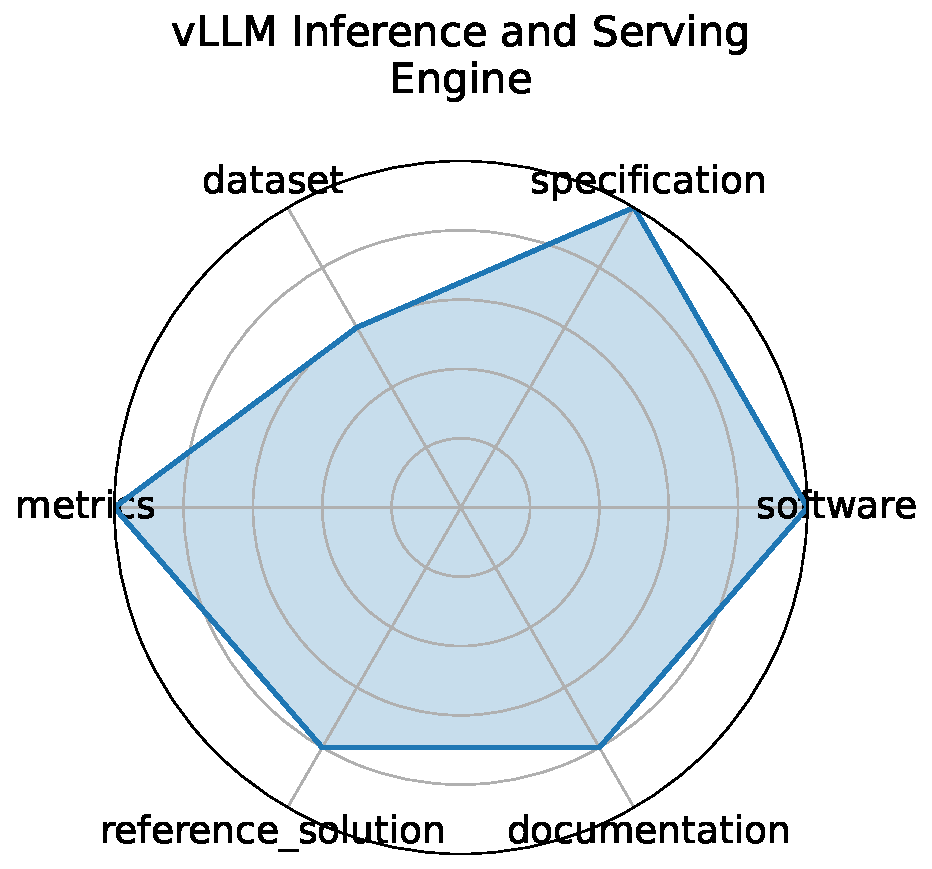
\includegraphics[width=0.2\textwidth]{vllm_inference_and_serving_engine_radar.pdf}
}}
\clearpage